\section{Context Viewpoint}

\subsection{View: Stakeholders}

\subsubsection{Model}
\begin{figure}[H]
    \centering
    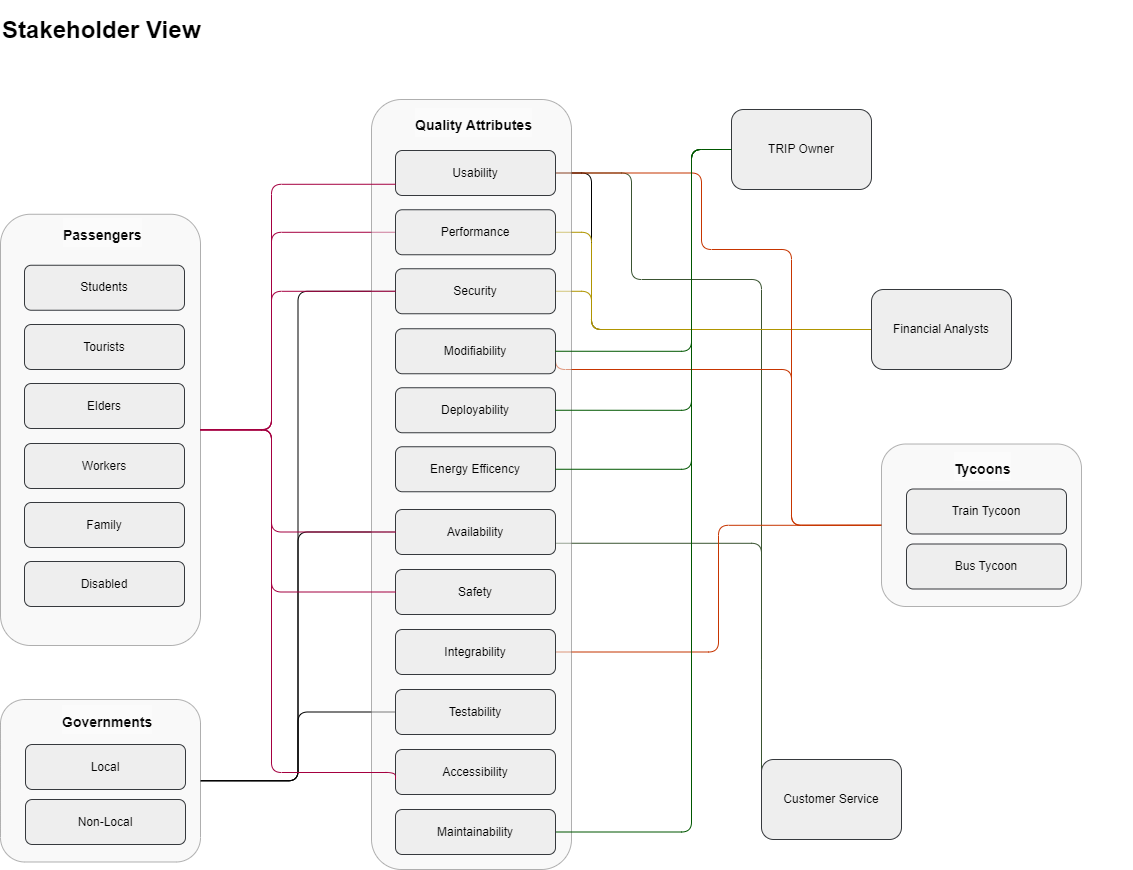
\includegraphics[width=\textwidth]{drawings/views_final_version/stakeholder_view.png}
    \caption{Stakeholder model of the TRIP system.}
    \label{fig:stakeholder_view_model}
\end{figure}

\subsubsection{Description}
The Stakeholder View of the TRiP System identifies the main participants and the corresponding quality attributes that are critical to their interaction with the system. Each stakeholder group—comprising Passengers, Tycoons, the TRiP Owner, Financial Analysts, Customer Service, and Governments—is associated with specific quality attribute depicted in the view.
\subsubsection{Glossary of Elements}
\begin{table}[H]
    \centering
    \begin{tabular}{@{}clp{9cm}@{}}
    \toprule
    \textbf{Id} & \textbf{Name} & \textbf{Description} \\
    \midrule
    1 & Passengers & Individuals or groups utilizing the TrIP system for travel, including diverse demographics such as students, tourists, workers, families, the elderly, and disabled persons. \\
    2 & Governments & Local and non-local government entities that oversee transportation regulations, public welfare, and infrastructure as it relates to the TrIP system. \\
    3 & Quality Attributes & Characteristics of the TrIP system valued by stakeholders, including usability, performance, security, modifiability, cost efficiency, availability, safety, integrability, and maintainability. \\
    4 & TRIP Owner & The entity or group of entities responsible for the oversight, strategic decision-making, and financial aspects of the TrIP system. \\
    5 & Financial Analysts & Professionals who assess the financial performance, cost-effectiveness, and economic impact of the TrIP system. \\
    6 & Tycoons & Operators or owners of train and bus services who use the TrIP system for fare collection, service management, and customer engagement. This includes both train tycoons and bus tycoons. \\
    7 & Customer Service & The support infrastructure that addresses passenger inquiries, resolves travel and payment issues, and enhances the overall customer experience within the TrIP system. \\
    \bottomrule
    \end{tabular}
    \caption{Glossary of stakeholder-related elements detailing the parties involved with the TrIP system and their interests.}
    \label{tab:glossary_stakeholder_view}
\end{table}


\subsection{View: Context diagram}
\subsubsection{Model}
\begin{figure}[H]
    \centering
    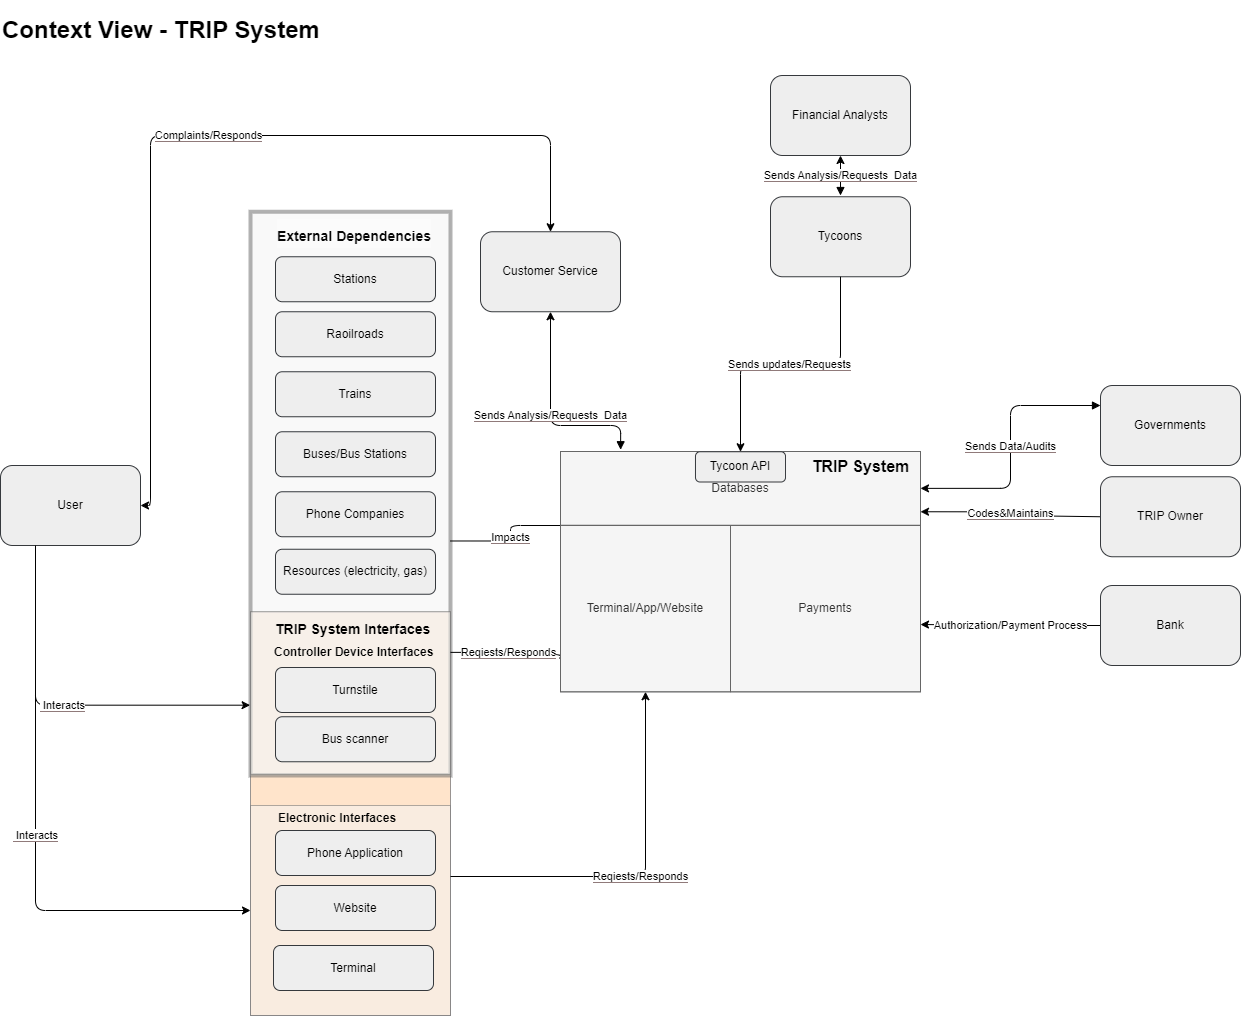
\includegraphics[width=\textwidth]{drawings/views_final_version/context_view.png}
    \caption{Context model of the TrIP system.}
    \label{fig:context_view_model}
\end{figure}

\subsubsection{Description}
The Context View of the TRiP SYSTEM delineates the ecosystem within which the system operates, including its interactions with users, external entities, and other system components. At the passenger level, engagement with the TRiP system is facilitated through various interfaces such as terminals, apps, websites, and controller devices like turnstiles and bus scanners, enabling passengers to access services seamlessly.

The system is subject to a range of external dependencies, including infrastructure elements like stations, railroads, and trains, as well as service providers such as phone companies and utilities that supply essential resources. These components are integral to the system's operations, impacting its functionality and performance.

At the core, the TRiP system is interconnected with Tycoons via the Tycoon API, through which data flows bidirectionally, allowing for the exchange of updates, requests, and analytical data. The databases within the system are pivotal in managing schedules, passenger accounts, tickets, and payments, all of which are crucial for the day-to-day operations.

The system's architecture is designed to ensure robustness and responsiveness to both the passengers' and Tycoons' needs. It facilitates various processes, from payment transactions, which are securely handled and routed through financial institutions, to the maintenance of service quality, overseen by the TRiP owner and regulated by governmental audits and codes. This comprehensive network of interactions defines the TRiP system's context, emphasizing its multifaceted nature and the critical role it plays in serving its stakeholders.

\subsubsection{Glossary of the Elements}
\begin{table}[H]
\centering
\begin{tabular}{@{}clp{9cm}@{}}
\toprule
\textbf{Id} & \textbf{Name} & \textbf{Description} \\
\midrule
1 & Passenger & Individuals who use the TrIP SYSTEM and its associated services, interacting through various interfaces. \\
2 & Customer Service & The department that handles passenger complaints and feedback, providing support and sending analysis or data requests to the system. \\
3 & Financial Analysts & Experts or entities that review financial data, requiring analytical information from the system for decision-making. \\
4 & Tycoons & The operational decision-makers of the system, possibly managers or algorithms that control system parameters and require data. \\
5 & Tycoon API & The programming interface through which Tycoons receive updates and send requests to the system. \\
6 & TrIP System & The core system that integrates various interfaces and processes, forming the central operation platform. \\
7 & Governments & Regulatory bodies that may require data or perform audits on the system for governance and compliance. \\
8 & TrIP Owner & The entity or person owning and maintaining the TrIP SYSTEM, responsible for its overall functionality. \\
9 & Bank & Financial institution that handles the authorization and processing of payments for the system. \\
10 & Stations & Locations where the TrIP SYSTEM provides service to passengers, such as train or bus stations. \\
11 & Railroads & Infrastructure providers that offer the tracks on which train services operate. \\
12 & Trains & The vehicles used by the system to transport passengers from one station to another. \\
13 & Buses/Bus Stations & The bus services and their stations that are part of the transport network. \\
14 & Phone Companies & Telecom service providers that facilitate mobile communication and data transfer for the system. \\
15 & Resources (electricity, gas) & Utility providers that supply essential power and energy required for the system’s operations. \\
16 & Controller Device Interfaces & The interfaces like turnstiles and bus scanners that manage access control and validate passenger credentials. \\
17 & Electronic Interfaces & Digital platforms such as mobile applications and websites that passengers interact with for services. \\
\bottomrule
\end{tabular}
\caption{Context model glossary for the TrIP System.}
\label{tab:glossary_context_view}
\end{table}
